\newpage
\phantomsection
\appendices
\appendix

\chapter{Matlab Code}
\label{Appendix A: Matlab Code}
\thispagestyle{pageonbottom}

\pagestyle{fancy}
\renewcommand{\sectionmark}[1]{\markright{#1}}
\fancyhead{}
%%%%%%%%%%%%%%%%%%%%%%%%%%%% The paper headers
\fancyhead[LE,RO]{\thepage}
\fancyhead[LO]{\text{Appendix A} \quad   {Matlab Code}}
\fancyhead[RE]{\text{Appendix A} \quad   {Matlab Code}} %Even page header and number at left top
\fancyfoot[L,R,C]{}
\renewcommand{\headrulewidth}{1pt}% disable the underline of the header part
%\end{flushleft}
We present a subset of the Matlab code used to simulate our numerical results. Three essential algorithms used to define the upper and lower fields are the computation of the flat--interface solution of $\bA_{0,0}$, the upper and lower layer DNOs, $G_{n,m}=G_{n,m}(x;\Eps,\delta)$ and $J_{n,m}=J_{n,m}(x;\Eps,\delta)$, and the upper and lower transformed field solvers, $u_{n,m}=$ $u_{n,m}(x,z;\Eps,\delta)$ and $w_{n,m}=w_{n,m}(x,z;\Eps,\delta)$. In Algorithm $\text{A}.0.1$ we show our technique for inverting the flat--interface solution of $\bA_{0,0}$ (cf. $\S 4.8$).
\vspace{-15mm}
\begin{algorithm}[H]
\caption{Inversion of the flat--interface operator $\bA_{0,0}$}
\label{alg:inverse_ao}
\begin{algorithmic}[1]
\State $\text{Set $Nx$: The number of discretization points}$
\State $\text{Set $i\gamma_p^u$: The Fourier multiplier for $G_{0,0}$}$
\State $\text{Set $i\gamma_p^w$: The Fourier multiplier for $J_{0,0}$}$
\State $\text{Set $\gamma^q=(1+\delta)\ugamma^q,q\in\{u,w\},$ where $\delta$ represents a small frequency perturbation}$
\State $\text{Set $\tau$: Constant representing TE or TM polarization mode}$
\State $\zeta_{0,0} \in\mathbb R^{N_x},~\psi_{0,0} \in\mathbb R^{N_x} $
\vspace{0.5mm}
\State $\widehat{\zeta}_{0,0} \in\mathbb C^{N_x},~\widehat{\psi}_{0,0} \in\mathbb C^{N_x} $
\For{$j=1:Nx$} \do ${\boldsymbol{\rightarrow} \text{Entries of $\left[ \widehat{\bA}_{0,0}(p) \right]^{-1} $}}$
\State $\operatorname{det}_p = -\left\{i\ugamma_p^u(j) + \tau^2\left( i\ugamma_p^w(j)\right)\right\}$
\State $\underline{a}(j) = \left[\tau^2\left( -i\ugamma_p^w(j)\right)\widehat{\zeta}_{0,0}(j) + \widehat{\psi}_{0,0}(j)\right]/\operatorname{det}_p $
\State $\underline{b}(j) = \left[\left(i\ugamma_p^u(j)\right)\widehat{\zeta}_{0,0}(j) + \widehat{\psi}_{0,0}(j)\right]/\operatorname{det}_p $
\EndFor
\State $U_{0,0}=\operatorname{IFFT}(\underline{a}), ~ W_{0,0}=\operatorname{IFFT}(\underline{b})$
\State\Return $U_{0,0}, W_{0,0}$
\end{algorithmic}
\end{algorithm}
\vspace{-17mm}
Next, Algorithm $\text{A}.0.2$ demonstrates how we calculate the upper layer DNO, $G$ (cf. $\S 2.10$ and $\S 2.11$).
\vspace{-14mm}
\begin{algorithm}[H]
\caption{Computation of the upper layer DNO, $G$}
\label{alg:dno}
\begin{algorithmic}[1]
\State $\text{Set $Nx$: The number of discretization points}$
\State $\text{Set $Nz$: The number of collocation points}$
\State $\text{Set $N$: The maximum number of Taylor orders for the interfacial perturbation}$
\State $\text{Set $M$: The maximum number of Taylor orders for the frequency perturbation}$
\State $\text{Set $dx$: The partial derivative with respect to the $x$ component}$
\State $\text{Set $dz$: The partial derivative with respect to the $z$ component}$
\State $\text{Set $a$: The artificial boundary imposed at the top of the upper layer}$
\algstore{myalg}
\end{algorithmic}
\end{algorithm}

\begin{algorithm}                     
\begin{algorithmic}[1]
\algrestore{myalg}
\State $\text{Set $\tilde{p}=(2\pi/d)p$ for an integer $p$ where $d$ is the periodicity of the grating interface}$
\State $\text{Set $f=\sin(x)$, or a similar test function representing the grating surface}$
\State $\text{Set $f_x:$ The derivative of $f$ with respect to the $x$ component}$
\State $\text{Set $\ell_{\text{bottom}}=Nz+1,$ the bottom or last collocation point on the $z$--axis}$
\State $u_{n,m}\in\mathbb C^{N_x\times (N_z+1) \times (M+1) \times (N+1)}, ~ G_{n,m} \in\mathbb C^{N_x\times (M+1) \times (N+1)} $
\State $u_x\in\mathbb C^{N_x \times (N_z+1)}, ~ u_z \in\mathbb C^{N_x \times (N_z+1)}$
\For{$n=1:N$}
\For{$m=1:M$} ${\boldsymbol{\rightarrow} \text{Order $(n,m)$ terms in equation $(2.52)$ in $\S 2.10 $}}$
\State $u_z = dz(u_{n,m}(:,:,m,n),a)$
\State $G_{n,m}(:,m,n) = -u_z(:,\ell_{\text{bottom}}) $
\If{$n > 1$} ${\boldsymbol{\rightarrow} \text{Order $(n-1,m)$ terms in equation $(2.53)$ in $\S 2.10 $}}$
\State $u_x = dx(u_{n,m}(:,:,m,n-1),\tilde{p})$
\State $G_{n,m}(:,m,n) = G_{n,m}(:,m,n) + f_xu_x(:,\ell_{\text{bottom}})$
\State $G_{n,m}(:,m,n) = G_{n,m}(:,m,n) + (1/a)\cdot (f\cdot G_{n,m}(:,m,n-1))$
\EndIf
\If{$n >2$} ${\boldsymbol{\rightarrow} \text{Order $(n-2,m)$ terms in equation $(2.53)$ in $\S 2.10 $}}$
\State $u_x = dx(u_{n,m}(:,:,m,n-2),\tilde{p})$
\State $G_{n,m}(:,m,n) = G_{n,m}(:,m,n) - (1/a)\cdot(ff_x\cdot u_x(:,\ell_{\text{bottom}}))$
\State $u_z = dz(u_{n,m}(:,:,m,n-2),a)$
\State $G_{n,m}(:,m,n) = G_{n,m}(:,m,n) - (f_x^2\cdot u_z(:,\ell_{\text{bottom}}))$
\EndIf
\EndFor
\EndFor
\State\Return $G_{n,m}$
\end{algorithmic}
\end{algorithm}
\vspace{-18mm}
Lastly, Algorithm $\text{A}.0.3$ summarizes how we compute the upper transformed field, $u$ (cf. $\S 2.4$, $\S 2.6$, and $\S 2.11$). Due to its complexity and length, we leave out some details to the Matlab implementation in Listing $\text{A}.1$. 
\vspace{-14mm}
\begin{algorithm}[H]
\caption{Computation of the upper transformed field, $u$}
\label{alg:transformed_field}
\begin{algorithmic}[1]
\State $\text{Set $Nx$: The number of discretization points}$
\State $\text{Set $Nz$: The number of collocation points}$
\State $\text{Set $N$: The maximum number of Taylor orders for the interfacial perturbation}$
\State $\text{Set $M$: The maximum number of Taylor orders for the frequency perturbation}$
\State $\text{Set $dx$: The partial derivative with respect to the $x$ component}$
\State $\text{Set $dz$: The partial derivative with respect to the $z$ component}$
\State $\text{Set $a$: The artificial boundary imposed at the top of the upper layer}$
\State $\text{Set $\tilde{p}=(2\pi/d)p$ for an integer $p$ where $d$ is the periodicity of the grating interface}$
\State $\text{Set $f=\cos(x)$, or a similar test function representing the grating surface}$
\State $\text{Set $f_x:$ The derivative of $f$ with respect to the $x$ component}$
\State $\text{Set $\ell_{\text{top}}=0+1,$ the top or first collocation point on the $z$--axis}$
\State $\text{Set $T^u:$ Expansion of frequency operator, cf. $\S 5.4$}$
\State $\text{Set $g(x)=\Eps f(x),$ where $\Eps$ represents a small interfacial perturbation}$
\State $\text{Set $\gamma^u=(1+\delta)\ugamma^u$, $\alpha = (1+\delta)\ualpha$,
where $\delta$ is a small frequency perturbation}$
\algstore{myalg_2}
\end{algorithmic}
\end{algorithm}

\begin{algorithm}[H]                    
\begin{algorithmic}[1]
\algrestore{myalg_2}
\State $\text{Set $z'=a(z-g(x))/(a-g(x)),$ per transformation rules in $\S 2.4.$ Relabel $z=z'$}$
\State $\xi_{n,m}\in\mathbb R^{N_x \times (M+1) \times (N+1)}, ~ \widehat{\xi}_{n,m}\in \mathbb C^{N_x \times (M+1) \times (N+1)} $
\State $U_{n,m}\in  \mathbb R^{N_x \times (N_z+1)},~ \widehat{U}_{n,m}\in  \mathbb C^{N_x \times (N_z+1)}$
\State $ F_{n,m}\in\mathbb R^{N_x \times (N_z+1)}, ~ \widehat{F}_{n,m}\in\mathbb C^{N_x \times (N_z+1)}$
\State $u_{n,m}\in\mathbb C^{N_x\times (N_z+1) \times (M+1) \times (N+1)}, ~J_{n,m}\in\mathbb R^{N_x}, ~ \widehat{J}_{n,m}\in\mathbb C^{N_x}$
\State $\text{Compute $A_1^{xx},A_1^{xz},A_1^{zx},A_1^{zz},A_2^{xx},A_2^{xz},A_2^{zx},A_2^{zz},B_1^{x},B_1^{z},B_2^{x},B_2^{z},S_0,S_1$, and}$
\State ${\text{$S_2$ through equations $(2.16)$ in $\S 2.4$}}$
\For{$n=1:N$}
\For{$m=1:M$}
\If{$n >  1$} ${\boldsymbol{\rightarrow} \text{Order $(n-1,m)$ terms in equation $(2.28)$ in $\S 2.6 $}}$
\State $u_x = dx(u_{n,m}(:,:,m,n-1),\tilde{p})$
\State $F_{n,m} = F_{n,m} - dx(A_1^{xx}\cdot u_x,\tilde{p})$
\State $F_{n,m} = F_{n,m} - dz(A_1^{zx}\cdot u_x,a)$
\State $F_{n,m} = F_{n,m} - B_1^{x}\cdot u_x$
\State $u_z = dz(u_{n,m}(:,:,m,n-1),a)$
\State $F_{n,m} = F_{n,m} - dx(A_1^{xz}\cdot u_z,\tilde{p})$
\State $F_{n,m} = F_{n,m} - (2i\ualpha)\cdot S_1 \cdot u_x $
\State $F_{n,m} = F_{n,m} - (\ugamma^u)^2\cdot S_1 \cdot u_{n,m}(:,:,m,n-1)$
\EndIf
\If{$m > 1$} ${\boldsymbol{\rightarrow} \text{Order $(n,m-1)$ terms in equation $(2.28)$ in $\S 2.6 $}}$
\State $u_x = dx(u_{n,m}(:,:,m-1,n),\tilde{p})$
\State $F_{n,m} = F_{n,m} - (2i\ualpha)\cdot u_x$
\State $F_{n,m} = F_{n,m} - (2(\ugamma^u)^2)\cdot u_{n,m}(:,:,m-1,n)$
\EndIf
\If{$n>1 \text{ and } m>1$} ${\boldsymbol{\rightarrow} \text{Order $(n-1,m-1)$ terms in equation $(2.28)$}}$
\State $u_x = dx(u_{n,m}(:,:,m-1,n-1),\tilde{p})$
\State $F_{n,m} = F_{n,m} - (2i\ualpha)\cdot S_1 \cdot u_x$
\State $F_{n,m} = F_{n,m} - (2(\ugamma^u)^2)\cdot S_1 \cdot u_{n,m}(:,:,m-1,n-1)$
\EndIf
\If{$n>2$} ${\boldsymbol{\rightarrow} \text{Order $(n-2,m)$ terms in equation $(2.28)$ in $\S 2.6 $}}$
\State $u_x = dx(u_{n,m}(:,:,m,n-2),\tilde{p})$
\State $F_{n,m} = F_{n,m} - dx(A_2^{xx}\cdot u_x,\tilde{p})$
\State $F_{n,m} = F_{n,m} - dz(A_2^{zx}\cdot u_x,a)$
\State $F_{n,m} = F_{n,m} - B_2^x \cdot u_x$
\State $u_z = dz(u_{n,m}(:,:,m,n-2),a)$
\State $F_{n,m} = F_{n,m} - dx(A_2^{xz} \cdot u_z,\tilde{p})$
\State $F_{n,m} = F_{n,m} - dz(A_2^{zz} \cdot u_z,a)$
\State $F_{n,m} = F_{n,m} - B_2^z \cdot u_z - (2i\ualpha)\cdot S_2 \cdot u_x$
\State $F_{n,m} = F_{n,m} - (\ugamma^u)^2 \cdot S_2 \cdot u_{n,m}(:,:,m,n-2)$
\EndIf
\algstore{myalg_2}
\end{algorithmic}
\end{algorithm}

\begin{algorithm}[H]                    
\begin{algorithmic}[1]
\algrestore{myalg_2}
\If{$m > 2$} ${\boldsymbol{\rightarrow} \text{Order $(n,m-2)$ terms in equation $(2.28)$ in $\S 2.6 $}}$
\State $F_{n,m} = F_{n,m} - (\ugamma^u)^2\cdot u_{n,m}(:,:,m-2,n)$
\EndIf
\If{$n>1 \text{ and } m > 2$} ${\boldsymbol{\rightarrow} \text{Order $(n-1,m-2)$ terms in equation $(2.28)$ }}$
\State $F_{n,m} = F_{n,m} - (\ugamma^u)^2 \cdot S_1 \cdot u_{n,m}(:,:,m-2,n-1)$
\EndIf
\If{$n > 2 \text{ and } m>1$} ${\boldsymbol{\rightarrow} \text{Order $(n-2,m-1)$ terms in equation $(2.28)$ }}$
\State $u_x = dx(u_{n,m}(:,:,m-1,n-2),\tilde{p})$
\State $F_{n,m} = F_{n,m} - (2i\ualpha)\cdot S_2 \cdot u_x$
\State $F_{n,m} = F_{n,m} - (2(\ugamma^u)^2) \cdot S_2 \cdot u_{n,m}(:,:,m-1,n-2)$
\EndIf
\If{$n>2 \text{ and } m > 2$} ${\boldsymbol{\rightarrow} \text{Order $(n-2,m-2)$ terms in equation $(2.28)$ }}$
\State $F_{n,m} = F_{n,m} - (\ugamma^u)^2 \cdot S_2 \cdot u_{n,m}(:,:,m-2,n-2)$
\EndIf
\For{$r=0:m-1$} ${\boldsymbol{\rightarrow} \text{Transparent boundary condition, $(2.29)$ in $\S 2.6$ }}$
\State $J_{n,m} = J_{n,m} + \operatorname{IFFT}( (T^u(:,m-r))\cdot \operatorname{FFT}(u_{n,m}(:,\ell_{\text{top}},r,n)))$
\EndFor
\If{$n > 1$}
\For{$r=0:m$} ${\boldsymbol{\rightarrow} \text{Transparent boundary condition, $(2.29)$ in $\S 2.6$ }}$
\State $S_{n,m} = \operatorname{IFFT}( T^u(:,m-r))\cdot \operatorname{FFT}(u_{n,m}(:,\ell_{\text{top}},r,n-1)) )$
\State $J_{n,m} = J_{n,m} - (1.0/a)\cdot f \cdot S_{n,m}$
\EndFor
\EndIf
\State $\widehat{F}_{n,m} = \operatorname{FFT}(F_{n,m}), ~ \widehat{J}_{n,m} = \operatorname{FFT}(J_{n,m})$
\State $\widehat{U}_{n,m} = \text{Chebyshev collocation method of parameters in $(2.63)$ of $\S 2.11$}$
\If{$n>0 \text{ or } m>0}$
\State $u_{n,m}(:,:,m,n)=\operatorname{IFFT}(\widehat{U}_{n,m})$
\EndIf
\EndFor
\EndFor
\State\Return $u_{n,m}$
\end{algorithmic}
\end{algorithm}
\vspace{-19mm}
We now turn to example Matlab implementations. Our first script is the code for the upper transformed field, $u=u(x,y;\varepsilon,\delta)$ (cf. Algorithm $\text{A}.0.3$). A computational novelty of our HOPS/AWE algorithm is the speed at which we can compute the flat--interface solution in Fourier space by inverting a sparse operator at every wavenumber. To do this, we apply the \gls{fft} and \gls{ifft} in Matlab. Because Matlab array indices start from $1$ (linear indexing), we will add ``$+1$'' in all of the loop variables executed in our Matlab scripts.

%\begin{singlespacing}
\begin{lstlisting}[caption={Upper Field Solver for the TFE Method},frame=single]
function [unm] = field_tfe_helmholtz_m_and_n(xi_n_m,f,p,gammap,alpha,...
        gamma,Dz,a,Nx,Nz,N,M,identy)

unm = zeros(Nx,Nz+1,M+1,N+1);

k2 = p(0+1)^2 + gammap(0+1)^2;

ell_top = 0 + 1;
xi_n_m_hat = 0*xi_n_m;
for n=0:N
  for m=0:M
    xi_n_m_hat(:,m+1,n+1) = fft(xi_n_m(:,m+1,n+1));
  end
end
f_x = real(ifft((1i*p).*fft(f)));

ll = [0:Nz]';
z_min = 0; z_max = a;
D = (2/(z_max-z_min))*Dz;
D2 = D*D;
D_start = D(1,:);
D_end = D(end,:);
tilde_z = cos(pi*ll/Nz);
z = ((z_max-z_min)/2.0)*(tilde_z - 1.0) + z_max;

f_full = repmat(f,1,Nz+1);
f_x_full = repmat(f_x,1,Nz+1);
a_minus_z_full = repmat(a - z.',Nx,1);

Uhat = zeros(Nx,Nz+1);

Tu = Tu_dno(alpha,p,gamma,gammap,k2,Nx,M);

% n=0 and m=0

for ell=0:Nz
  unm(:,ell+1,0+1,0+1) = ifft(exp(1i*gammap*z(ell+1)).*xi_n_m_hat(:,0+1,0+1));
end

A1_xx = -(2.0/a)*f_full;
A1_xz = -(1.0/a)*(a_minus_z_full).*f_x_full;
A1_zx = A1_xz;
%A1_zz = 0;
  
A2_xx = (1.0/a^2)*f_full.^2;
A2_xz = (1.0/a^2)*(a_minus_z_full).*(f_full.*f_x_full);
A2_zx = A2_xz;
A2_zz = (1.0/a^2)*((a_minus_z_full).^2).*(f_x_full.^2);
  
B1_x = (1.0/a)*f_x_full;
%B1_z = 0;
  
B2_x = -(1.0/a^2)*f_full.*f_x_full;
B2_z = -(1.0/a^2).*(a_minus_z_full).*(f_x_full.^2);

S1 = -(2.0/a)*f_full;
S2 = (1.0/a^2)*f_full.^2;

for n=0:N
  for m=0:M
    
    % Form Fnm, Jnm
    Fnm = zeros(Nx,Nz+1);
    Jnm = zeros(Nx,1);
    
    if(n>=1)
      u_x = dx(unm(:,:,m+1,n-1+1),p);
      temp = A1_xx.*u_x;
      Fnm = Fnm - dx(temp,p);
      temp = A1_zx.*u_x;
      Fnm = Fnm - dz(temp,Dz,a);
      temp = B1_x.*u_x;
      Fnm = Fnm - temp;
    
      u_z = dz(unm(:,:,m+1,n-1+1),Dz,a);
      temp = A1_xz.*u_z;
      Fnm = Fnm - dx(temp,p);
      %A1_zz = 0
      %B1_z = 0
    
      temp = 2*1i*alpha.*S1.*u_x;
      Fnm = Fnm - temp;
	  temp = gamma^2.*S1.*unm(:,:,m+1,n-1+1);
	  Fnm = Fnm - temp;
    end
	
 	if(m>=1)
 	  u_x = dx(unm(:,:,m-1+1,n+1),p);
 	  temp = 2*1i*alpha.*u_x;
 	  Fnm  = Fnm - temp;
 	  temp = 2*gamma^2.*unm(:,:,m-1+1,n+1);
 	  Fnm  = Fnm - temp;
 	end
	
 	if(n>=1 && m>=1)
 	  u_x = dx(unm(:,:,m-1+1,n-1+1),p);
 	  temp = 2*1i*alpha.*S1.*u_x;
 	  Fnm  = Fnm - temp;
 	  temp = 2*gamma^2.*S1.*unm(:,:,m-1+1,n-1+1);
 	  Fnm  = Fnm - temp;
 	end
	 
    if(n>=2)
      u_x = dx(unm(:,:,m+1,n-2+1),p);
      temp = A2_xx.*u_x;
      Fnm = Fnm - dx(temp,p);
      temp = A2_zx.*u_x;
      Fnm = Fnm - dz(temp,Dz,a);
      temp = B2_x.*u_x;
      Fnm = Fnm - temp;
    
      u_z = dz(unm(:,:,m+1,n-2+1),Dz,a);
      temp = A2_xz.*u_z;
      Fnm = Fnm - dx(temp,p);
      temp = A2_zz.*u_z;
      Fnm = Fnm - dz(temp,Dz,a);
      temp = B2_z.*u_z;
      Fnm = Fnm - temp;
    
      temp = 2*1i*alpha.*S2.*u_x;
      Fnm = Fnm - temp;
	  temp = gamma^2.*S2.*unm(:,:,m+1,n-2+1);
	  Fnm = Fnm - temp;
    end
	
    if(m>=2)
 	  temp = gamma^2.*unm(:,:,m-2+1,n+1);
 	  Fnm = Fnm - temp;
    end
 	
    if(n>=1 && m>=2)
 	 temp = gamma^2.*S1.*unm(:,:,m-2+1,n-1+1);
 	 Fnm = Fnm - temp;
    end
 	
    if(n>=2 && m>=1)
 	 u_x = dx(unm(:,:,m-1+1,n-2+1),p);
 	 temp = 2*1i*alpha.*S2.*u_x;
 	 Fnm = Fnm - temp;
 	 temp = 2*gamma^2.*S2.*unm(:,:,m-1+1,n-2+1);
 	 Fnm = Fnm - temp;
    end
 	
    if(n>=2 && m>=2)
 	 temp = gamma^2.*S2.*unm(:,:,m-2+1,n-2+1);
 	 Fnm = Fnm - temp;
    end
     
    for r=0:m-1
      Jnm = Jnm + ifft((Tu(:,m-r+1)).*fft(unm(:,ell_top,r+1,n+1)));
    end
    if(n>=1)
      for r=0:m
        Snm = ifft((Tu(:,m-r+1)).*fft(unm(:,ell_top,r+1,n-1+1)) );
        Jnm = Jnm - (1.0/a)*f.*Snm;
      end
    end
    
    % Solve elliptic equation
    
    Fnmhat = fft(Fnm);
    Jnmhat = fft(Jnm);
    
    b = Fnmhat.';
    alphaalpha = 1.0;
    betabeta = 0.0;
    gammagamma = gamma*gamma - p.^2 - 2*alpha.*p;
    d_min = 1.0;
    n_min = 0.0;
    r_min = xi_n_m_hat(:,m+1,n+1);
    d_max = -1i*gammap;
    n_max = 1.0;
    r_max = Jnmhat;
    
    % Solve BVP through the Chebyshev collocation method
    
    Uhat = solvebvp_colloc(Uhat,b,alphaalpha,betabeta,gammagamma,...
        d_min,n_min,r_min,d_max,n_max,r_max,Nx,identy,D,D2,D_start,D_end);
    
    if((n>0)||(m>0))
      unm(:,:,m+1,n+1)=ifft(Uhat);
    end
    
  end
end

return;
\end{lstlisting}
%\end{singlespacing}
Our next script shows how we use the boundary data from the upper field solver to calculate the transformed field in Fourier space. We recover field data by inverting this operation for every perturbation order of $\varepsilon$ and $\delta$.

%\begin{singlespacing}
\begin{lstlisting}[caption={BVP Solver for the Chebyshev Collocation Method},frame=single]
function [Uhat] = solvebvp_colloc(Uhat,b,alpha,beta,gamma,d_min,n_min,...
    r_min,d_max,n_max,r_max,Nx,identy,D,D2,D_start,D_end)

A = alpha*D2 + beta*D + reshape(gamma,1,1,Nx).*identy;
A(end,:,:) = repmat(n_min*D_end,[1,1,Nx]);
b(end,:) = r_min;
      
A(1,:,:) = repmat(n_max*D_start,[1,1,Nx]);
A(end,end,:) = A(end,end,:) + d_min;
A(1,1,:) = A(1,1,:) + reshape(d_max,1,1,Nx);
b(1,:) = r_max;

for j=1:Nx
   utilde = linsolve(A(:,:,j),b(:,j)); % A\b
   Uhat(j,:) = utilde.';
end

return;
\end{lstlisting}
%\end{singlespacing}
Linsolve (or, equivalently, the backslash operator) is the most computationally expensive part of our algorithm. We can increase the computational speed through making the following changes in the Parallel Computing Toolbox in Matlab. Further improvements could be made by switching to a compiled programming language such as C\texttt{++}, Fortran, or Julia.
%\begin{singlespacing}
\begin{lstlisting}[caption={Parallel Version of the BVP Solver for the Chebyshev Collocation Method},frame=single]
% Execute for-loop iterations in parallel on workers
parfor j=1:Nx
   utilde = linsolve(A(:,:,j),b(:,j)); % A\b
   Uhat(j,:) = utilde.';
end

% Remove the for loop by mldivide with GPU arrays
Uhat = permute( pagefun(@mldivide,A,reshape(b,[],1,Nx)),[2,1,3]);
\end{lstlisting}
%\end{singlespacing}
We note that these changes are only necessary for large simulations (such as $N=M=15$ or more Taylor orders and a granularity of $N_{\delta}=N_{\varepsilon}=1000$ per invocation, cf. $\S 6.3$ and $\S 6.5$). The additional overhead and partitioning for parallel workers or the GPU is unwarranted for smaller simulations which can often be computed in a few minutes or less. Our next script shows how we calculate the upper layer DNO through our TFE methodology (cf. Algorithm $\text{A}.0.2$).
%\begin{singlespacing}
\begin{lstlisting}[caption={Upper Layer DNO for the TFE Method},frame=single]
function [Gnm] = dno_tfe_helmholtz_m_and_n(unm,f,p,Dz,a,Nx,Nz,N,M)

Gnm = zeros(Nx,M+1,N+1);

ell_bottom = Nz + 1;
f_x = ifft((1i*p).*fft(f));

for n=0:N
  for m=0:M
    u_z = dz(unm(:,:,m+1,n+1),Dz,a);
    Gnm(:,m+1,n+1) = -u_z(:,ell_bottom);
    if(n>=1)
      u_x = dx(unm(:,:,m+1,n-1+1),p);
      Gnm(:,m+1,n+1) = Gnm(:,m+1,n+1) + f_x.*u_x(:,ell_bottom);
    
      Gnm(:,m+1,n+1) = Gnm(:,m+1,n+1) + (1.0/a)*(f.*Gnm(:,m+1,n-1+1));
    end
    if(n>=2)
      u_x = dx(unm(:,:,m+1,n-2+1),p);
      Gnm(:,m+1,n+1) = Gnm(:,m+1,n+1) - (1.0/a)*(f.*(f_x.*u_x(:,ell_bottom)));

      u_z = dz(unm(:,:,m+1,n-2+1),Dz,a);
      Gnm(:,m+1,n+1) = Gnm(:,m+1,n+1) - f_x.*(f_x.*u_z(:,ell_bottom));
    end
  end
end

return;

\end{lstlisting}
\vspace{-1mm}
We then demonstrate how to invert $\bA_{0,0}$ by Fourier inversion (cf. Algorithm $\text{A}.0.1$) where we multiply the numerator and denominator by $i$.
%\end{singlespacing}


\begin{lstlisting}[caption={Inversion of Flat--Interface $\bA_{0,0}$},frame=single]
function [U,W] = AInverse(Q,R,gammap,gammapw,Nx,tau2)
% Q = Zeta_{0,0}, R = Psi_{0,0}
  
a = zeros(Nx,1);
b = zeros(Nx,1);
Q_hat = fft(Q);
R_hat = fft(R);

for j=1:Nx
  det_p = tau2*gammapw(j) + gammap(j);
  a(j) = ((tau2*gammapw(j))*Q_hat(j) + 1i*R_hat(j))/det_p;
  b(j) = ((-gammap(j))*Q_hat(j) + 1i*R_hat(j))/det_p;
end

U = ifft(a);
W = ifft(b);

return;
\end{lstlisting}
\vspace{2mm}
Finally, in Figures $36$ and $37$, we show how Spectral methods are implemented in Matlab. Recalling our strategy in $\S 2.11$, we enforce a Fourier spectral method in the $x$--axis with $N_x$ equally--spaced gridpoints and a Chebyshev spectral method in the $z$--axis with $N_z + 1$ collocation points where, for brevity, we demonstrate our methods with $N_x=N_z=8$.
\vspace{-16mm}
\begin{figure}[H]
    \centering
    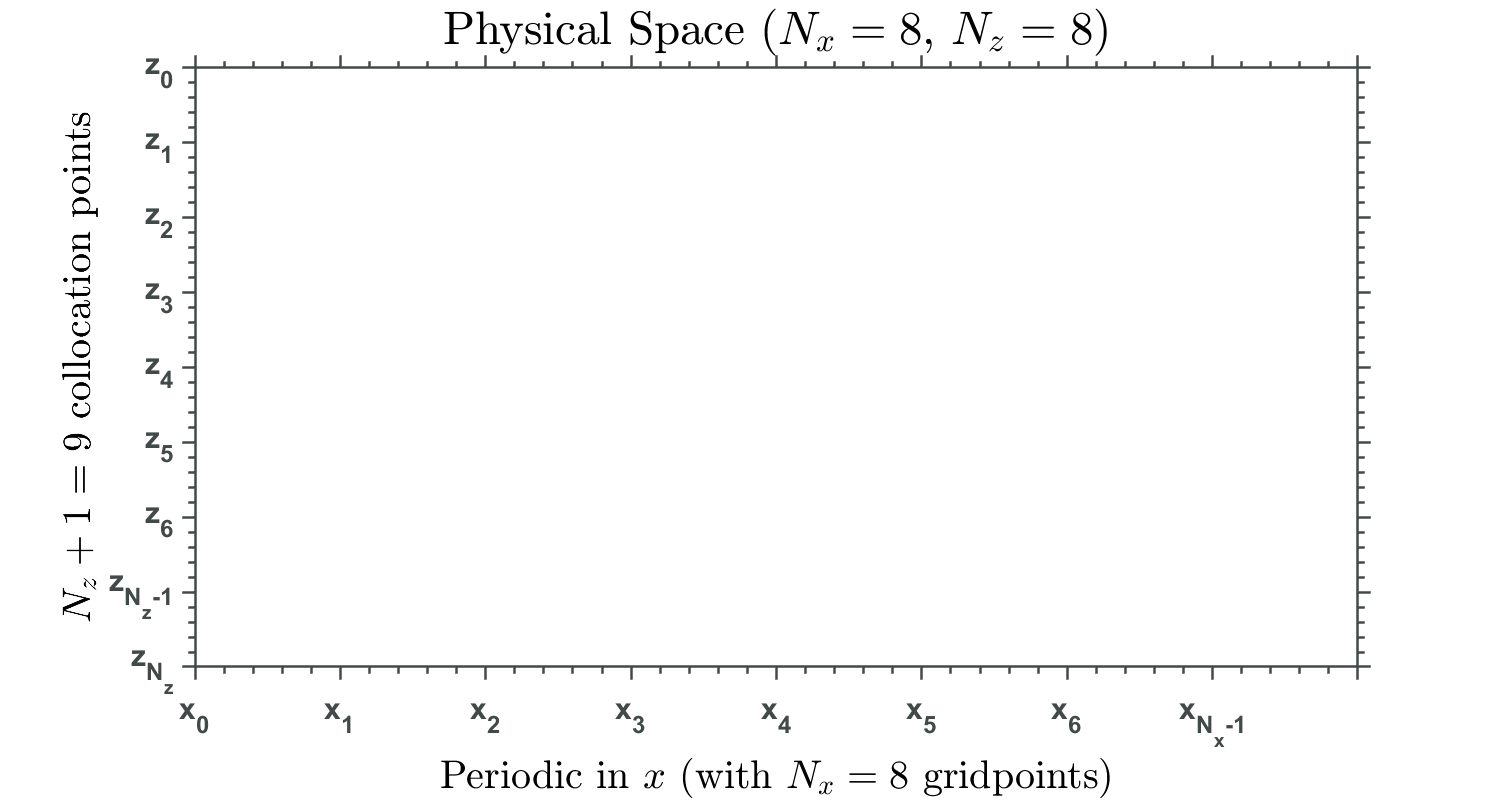
\includegraphics[width=16cm,height=16cm,keepaspectratio]{sections/other/matt_1.png}%
    \vspace{1mm}
    \caption{In Physical Space, we consider $N_x$ discretization points on the $x$--axis \\and $N_z+1$ collocation points on the $z$--axis.}%
    \label{fig:physical_space}%
\end{figure}


\vspace{-18mm}
\begin{figure}[H]
    \centering
    %\hspace{-15mm}
    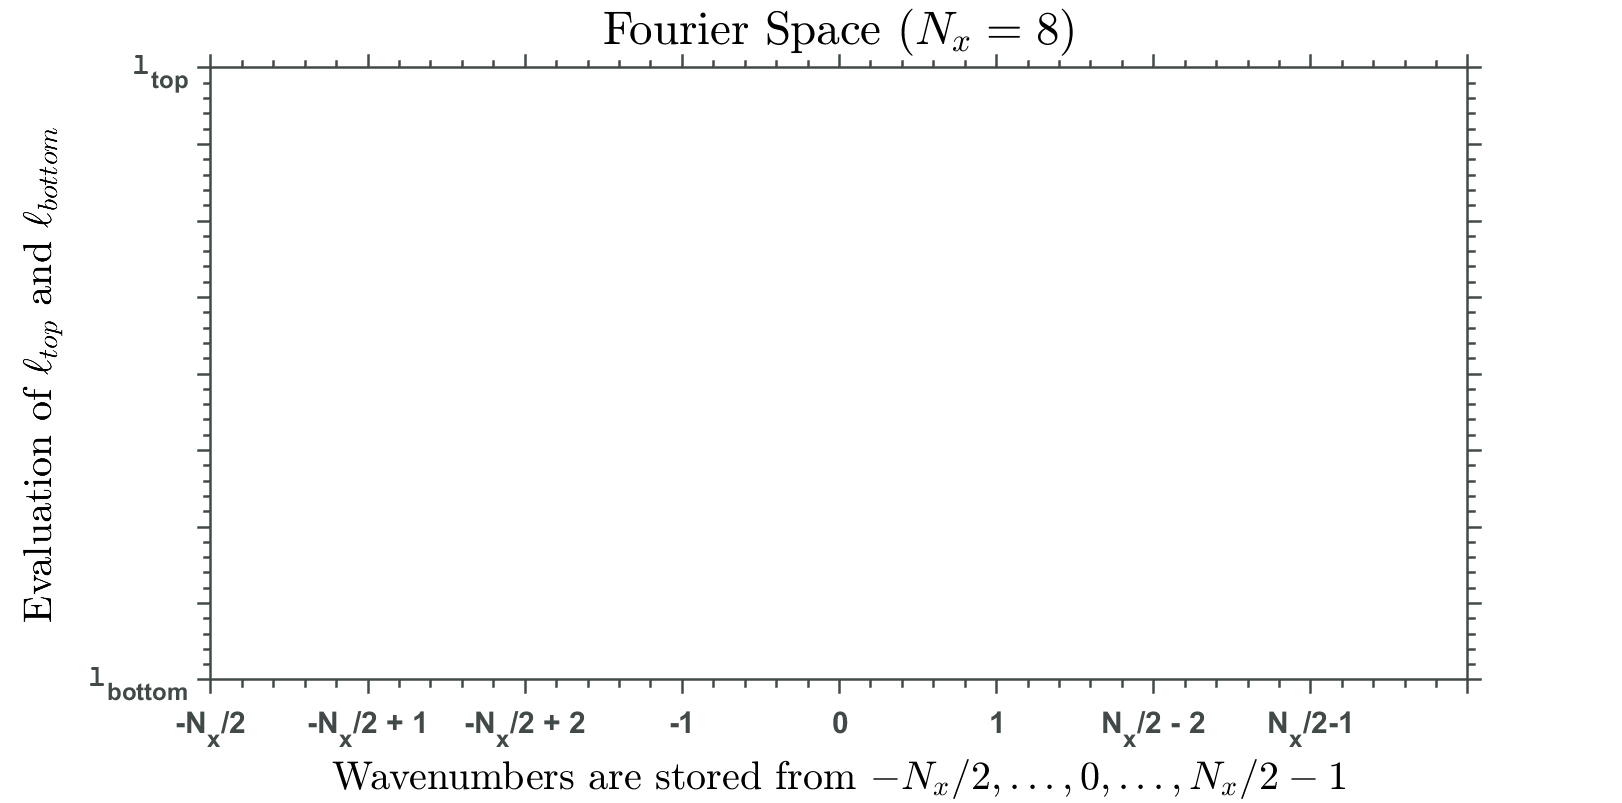
\includegraphics[width=16cm,height=16cm,keepaspectratio]{sections/other/matt_2.png}%
    \vspace{3mm}
    \caption{In Fourier Space, wavenumbers are stored in the order $-N_x/2,$ $\ldots,0,\ldots,N_x/2-1$ and $\ell_{top}$ and $\ell_{bottom}$ are evaluated at the upper boundary $z=a$ and the surface $z=0$ (cf. Algorithm $\text{A}.0.2$ and $\text{A}.0.3$).}
    \label{fig:fourier_space}%
\end{figure}
\vspace{-15mm}
More generally, we consider the Fourier transform on the $N_x$--point grid with a period of $d$. For $N_x$ discretization points and a step size of $(d/N_x)$, we have
\begin{align*}
\text{Physical ~Space :}&~~x\in\Big\{0,\
\frac{d}{Nx},\frac{2d}{Nx},\ldots,\frac{(N_x-2)d}{N_x},\frac{(N_x-1)d}{N_x}\Big\}   \\
\text{Fourier ~Space :}& ~~p\in\Big\{-\frac{N_x}{2},-\frac{N_x}{2}+1,\ldots,\frac{N_x}{2}-2,\frac{N_x}{2}-1\Big\}
\end{align*}
where the \gls{dft} is computed through several applications of the Fast Fourier Transform (FFT).